\documentclass[10pt,twoside]{report}
\usepackage[utf8]{inputenc}
\usepackage[nottoc]{tocbibind}              % append the reference to the table of content
\usepackage{times}
\usepackage{setspace}
\usepackage{booktabs}
\usepackage{graphicx}
\usepackage{amsmath}
\graphicspath{{images/}}
\usepackage[a4paper,width =150mm,top=25mm,bottom=25mm]{geometry}
\usepackage{fancyhdr}
\usepackage{pdfpages}
\usepackage{float}
\fontsize{7pt} {7.2}\selectfont
\pagestyle{fancy}
\fancyhf{}
\fancyhead[LE,RO]{\leftmark}
\fancyhead[RE,LO]{\rightmark}
\fancyfoot[CE,CO]{Indian Institute of Space Science and Technology, Trivandrum }
\fancyfoot[LE,RO]{\thepage}
\renewcommand{\headrulewidth}{2pt}
\renewcommand{\footrulewidth}{1pt}

\usepackage{biblatex}
\addbibresource{references.bib}
\usepackage[ruled,vlined]{algorithm2e} % used for algorithm formatting


% title section
\title{Thesis Title}
\author{Author Name}
\pagenumbering{roman}
\doublespacing

\begin{document}                   % document begin
\input{titlepage.tex}

\tableofcontents
\listoffigures


\chapter{Literature Survey}
\pagenumbering{arabic}
\chapter{Literature review}
\label{literature}

\section{Introduction}
The primary constraint in Aerodynamics Shape Optimization (ASO) is objective function evaluations, which are computationally expensive. This requires optimized methods to reduce the objective function evaluations. Apart from this, the other concern is to parameterize the wing and the choice of design variables. ADODG has suggested a problem (case 6) that involves investigating the existence of multimodality in NACA0012 wing subjected to geometric and aerodynamics constraints. Subsequent sections summarizes the work involving the parameterization of an object's shape and the algorithms to find multi-modal optima within the given design space.

\section{Historical work}

Chernukhin \cite{oleg} investigated the existence of multimodality in aerodynamic design space. The author proposed two novel optimization algorithms that can be used to find the existence of multimodality. They are gradient-based multi-start optimization (GB-MS) based on Sobel sampling and the genetic algorithm. These algorithms are initially tested on the 2-D ASO problem. Using the gradient-based method, the optimizer took 64000 functions evaluation to converge to single optima. However, carry out these many function evaluations would require a lot of computational time. Also, the design space chosen appears to be huge.

Further, the author extends the work to 3-D ASO (similar to that of ADODG case 6), with both transonic and subsonic conditions. The volume mesh is made of 12 blocks with 1.1m nodes. The objective function is to minimize the drag at a Mach number of 0.8 and lift constrained 0.2625. The wing is parameterized using a 2-patch B-spline surface with an initial NACA 0012 baseline wing having a rectangular crossover and a semi span of two. With 125 design variables, the GB optimizer took 60 function evaluations. A similar approach is carried out with GB-MS method involving 128 initial geometries resulting in single optima. In subsonic conditions, that is with Mach number 0.5 and angle of attack between -3 and +6 degree, resulted in seven unique local optima whose objective values differ by more than 5\%. 

The author confirms that 2-D airfoil optimization is unimodal, whereas 3-D wing optimization in subsonic flow conditions is multimodal \cite{oleg:phd}. However, with additional geometric constraints may further reduce multimodality. This work uses the GB-MS algorithm, and gradient-based methods are generally sensitive to the initial population. Also, the use of a gradient-free algorithm in large design variables is computationally expensive and unacceptable. However, with reduced design variables, it is possible to use a gradient-free method efficiently.


In work published by D.J. Poole \cite{Poole1} $et$ $al$., the author addressed the ADODG case 6 problem. The problem is to minimize the drag subjected to aerodynamics and geometric constraints. The wing is of rectangular section with a span length of 3 units and round winglet of 0.06 units. Also, the wing is subjected to compressible, inviscid flow with a Mach number of 0.5 and a constrained lift coefficient of 0.2625. The volume mesh is made of structured multiblock with the convective term being evaluated using Jameson-Schmidt-Turkel (JST) scheme. Nearly 5.5m node points are generated in an eight-block structured C-mesh topology. Further, the surface mesh is made of 129 $\times$ 41 mesh points. The author recommends using radial basis functions (RBFs) for surface control and mesh deformations.

The wing is parameterized using five equally spaced layers along the span direction comprising of 24 control points each along the chord direction. In total, the problem contains 22 design variables with thickness,  z-position, x-position, and a chord at five equally spaced wing sections, resulting in 20 design variables. The remaining two design variables are AoA and Twist [zero at the root and twist angle at the tip]. The AoA is varied within limits set by constraints. The author utilized a hybrid optimizer consisting of particle swarm optimization (PSO) and gravitational search algorithm (GSA). 

The work contains three cases; thickness optimization only, chord optimization only, and full optimization. However, the algorithm which is adopted here result in global optimization. Achieving multimodality is not possible with these algorithms. It is found that the design space chosen for full optimization is multimodal. A strong coupling exists between the chord and thickness of the wing, which increases the multimodality of the problem. However, the existence of multimodality is confirmed by running the optimizer several times. This allows the researcher to rethink on optimizer, which proves multimodality in a single run.

It can be concluded that for any ASO problems, the crucial steps involved are a choice of parameterization technique, selection of optimizer, and the optional step involving dimensional reduction method. Upcoming sections cover the historical work which involve the parameterization techniques, and selection of optimizer.

In the past, attempts have been made to simplify the geometry representation. Meaux $et$  $al$. \cite{Meaux} used (Non-Uniform Rational B-Spline) NURBS to optimize complex 3D geometries. Nadarajah\cite{Nadarajah} compares three different \textbf{parameterization schemes}: B-splines, CST method, and Mesh-point for airfoil geometry. The Mesh-point method involves representing the wing shape with x, y, and z coordinates of grid points. This method would be inefficient as it takes mesh points coordinates as design variables. Since this method involves large matrix operation, evaluating the gradient is difficult, which limits the use of descent algorithm. In the B-spline method, the degree of polynomial representing the surface act as a design variable. With a lower degree to polynomial, it is possible to reduce the dimension of the optimization problem.

The CST method provides the mathematical description of the geometry through a combination of a shape function and class function. The class function provides for a wide variety of geometries. The shape function replaces the complex non-analytic function with a simple analytic function. The simple analytical function uses only a scalable parameter to represent a large domain of design space for the aerodynamic problem. The advantage of CST is, it is efficient in terms of a low number of design variables and allows the use of industrial-related design parameters like the radius of the leading edge or maximum thickness and location\cite{Nadarajah}. The author has shown that the B-spline method allows fewer design variables to represent the wing surface. Due to its low number of design variables, gradient-free methods can be implemented. The complexity involved in the CST method prevents the researcher from using it. 

Gradient-free methods are generally adopted for unconstrained optimization problems. Additional steps need to be followed to implement constraints. One of them is constraint handling as proposed by Deb and Saha \cite{Deb}. The author D.J Poole \cite{Poole2} refers to the constraint handling technique proposed by Deb. Additionally, the author introduces the parallel decomposition of the niching DE algorithm tested on benchmark functions and are reliable.

The author D.J Poole \cite{Poole3} introduced a total of 18 benchmark functions to test the DE-based niching method. Among them, nine are from literature, and remaining are from his work. Along with benchmark functions, different niching methods are also published. The author has shown that, niching methods based on \textbf{neighbourhood search} show better results in terms of quick convergence and reliability of stable niches. However, these algorithms require an extensive amount of cost function evaluations. Hence some modification is necessary to implement them on ASO.

\section{Conclusion}
After analyzing over a few historical work, it can be said that further investigation over finding multimodality is necessary. The work presented by Chernukhin involves parameterization of the wing using B-spline surfaces. However, parameterization techniques called free-form deformation (FFD) can be adopted. The FFD is easy to implement. In case if the design variable appears more in number, then reduced-order modelling methods can be implemented, which will reduce the dimension of the problem by a significant amount.

This work focuses on using the niching algorithms to obtain all possible optima. The niching techniques balance the population diversity by modifying selection, mutation, or crossover stages of Canonical DE. Since they construct on DE, the convergence rate is slow. When combined with these algorithms, the GB method will make them become fast, resulting in Hybrid optimization. The solution is expected to converge faster. The DE based parallel niching algorithms provide a better solution to these class of problems. The scale factor $F$ and cross-factor $ CR $ have a significant impact on the algorithm's performance, such as the quality of the optimal value and convergence rate. There is still no ideal way to determine parameters\cite{chen}. The quality of mesh that is used in D.J.Poole work is super fine. However, with the available computational power, following such a high-quality grid seems complicated. 

According to Chernukhin \cite{oleg}, surrogate modelling is challenging to handle when the number of design variables becomes large. The 3D wing optimization with a viscous model not covered in the paper. However, this involves vast resources to optimize. With the available resources, it becomes difficult to handle. Little work has taken place in optimizing the wing with pre-defined winglet shape. The niching techniques involve a considerable quantity of cost function evaluations. So there needs to reduce cost function evaluation by modifying the code. In the end, solving the ADODG case 6 problems with FFD parameterization, combined with reduced-order modelling and the niching algorithms would lead to a new dimension to approach this problem.   % chapter one

\chapter{Niching Method}               % chapter two
\chapter{Niching Algorithms}
\label{niching}
\section{Background}
Aerodynamic shape optimization (ASO) is defined as finding the shape that optimizes a performance quantity subject to drag, geometrical constraints. Much of the work carried out in the past involved finding the single best optimum solution. However, during the design process, identifying other optimal designs may positively impact the cost and performance. Many aerodynamics optimization problems can be unimodal or multimodal. The parallel niching optimization algorithms direct the given multimodal optimization problem to identify the multiple optima in the given design space. This chapter contains a detailed explanation of the differential evolution (DE) based parallel niching algorithms.

 The DE algorithms are defined to find global optima for a given scalar objective function $f\mathbf{(x_i)}$ where, $\mathbf{x_i}$ is a design variables such that \textbf{i} $\in[1,\ldots,N]$ and \textbf{x} $\in{\mathcal{R}^D}$ with $D$ being problem dimension and $N$ being total population. Also, the DE algorithms are designed for unconstrained optimization problems. However, most of the real-world problems involve some constraints. In such a case, the DE algorithm needs to be modified. These modifications involve introducing a penalty method that results in a class of problems called \textbf{Multimodal optimization problem}.

Furthermore, the modifications to the DE algorithm are referred to as \textbf{Niching Algorithms}. These techniques will enhance the population’s diversity by locating the optimal solution in different parts of the design space. A considerable amount of research has taken place in constraint handling and multimodal optimization using nature-inspired algorithms. Upcoming sections contain a detailed explanation of DE and the modification to algorithms.
\section{Differential Evolution}
DE is a population-based optimization algorithm, where operators for mutation, crossover, and selection act to create a new population from an existing one. Eventually, through a series of iterations, the population will converge on to a globally optimal solution \cite{Poole3}. The DE is suitable for problems with discontinuous objectives, also with a problem having multiple local optima (multimodality). However, DE has slow convergence. Nearly 200 times more functional evaluations are required for Gradient-free methods as compared to gradient-based methods \cite{oleg}.

The DE is a parallel direct search method which utilizes $N$
D-dimensional design vectors \textbf{x$_{n,G}$}, where n = 1, 2, ... , N and g is the generation ranging between $[1, G]$. $N$ does not alter during the optimization
process. The initial population is chosen randomly and should cover the entire design space. As a rule, it is assumed to follow a uniform probability distribution for all random decisions unless otherwise stated. In case a preliminary solution is available, the initial population might be generated by adding normal distributed random deviations to the nominal solution $\textbf{x}_{nom,0}$. The DE generates another vectors by adding the weighted difference between two population vectors to a third vector. This operation is called \textit{mutation}.

The mutated vector individuals are merged with the individuals of another predetermined vector, the target vector, to generate the \textit{trial vector}. This operation is referred to as "\textit{crossover}." If the trial vector yields a lower cost function value than the target vector, the trial vector replaces the target vector in the following generation. This last operation is called "\textit{selection}". Each population vector has to serve once as the target vector so that $ N $ competitions occur in a given generation \cite{storn}.

The mathematical representation of the DE algorithm is explained as follows.
\begin{enumerate}
\item \underline{Initialization}: Here the initial population $N$ is generated randomly as: 
\begin{equation}
\textbf{x}_{n,g}^{d}=\textbf{L}^{d}+\operatorname{rand}(0,1)\left(\textbf{U}^{d}-\textbf{L}^{d}\right)
\label{initlize}
\end{equation}
where $rand(0, 1)$ is a uniformly distributed random number on the interval [0, 1]. $L^d$ and $U^d$ represents the lower and the upper limits of the design space respectively. And, $d$ is dimension of problem which can be $(d\in\{1, \ldots, D\}))$.

\item \underline{Mutation}: For each individual in the population, corresponding donor vector is generated as follows: initially, the weighted difference is taken between two randomly selected individuals from population,then it is added it to base vector (\textbf{x}$_{b,G}$). There are several strategies proposed that define the base vector. If in case DE/best/1 strategy is chosen, then the \(n\)-th donor vector is represented using equation \ref{best_mutation}. 
\begin{equation}
\mathbf{v}_{n}=\mathbf{x}_{b}(t)+F\left(\mathbf{x}_{r_{1}}(t)-\mathbf{x}_{r_{2}}(t)\right)
\label{best_mutation}
\end{equation}
$$
b=\underset{i \in\{1, \ldots, N\}}{\arg \min } f\left(\mathbf{x}_{i}\right)
$$
where, $F$ is the scaling factor ranging between [0, 1]. A higher scaling factor may force the donor individual to fall out of design space. Whereas, the lower value will generate the donor vector close to target individual. A value of $F = 0.5$ is considered to be a good trade off. $x_{b,g-1}$ is the best individual from the previous generation. $r_1$ and $r_2$ are uniformly distributed random integers in the interval [1, N] such that \(r_{1} \neq r_{2} \neq b\) and \(r_{1} \neq r_{2} \neq n\). A better representation of mutation stage in 2-D design space is shown in figure \ref{mutation}.
\begin{figure}[!ht]
    \centering
    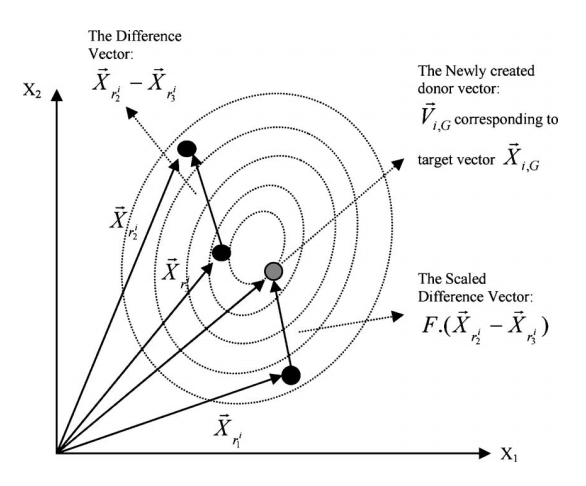
\includegraphics[scale = 0.5]{figures/mutation.png}
    \caption{2-D design space representing mutation stage \cite{storn}.}
    \label{mutation}
\end{figure}

\item \underline{Cross-over}: In this stage, elements from the target vector and donor vector are combined in a specific order to get a trial vector (\textbf{u}$_{n,g}$). This process is referred as binomial crossover. This stage play a vital role in increasing the population's diversity, and is shown in equation \ref{cross-over}.

\begin{figure}[!ht]
    \centering
    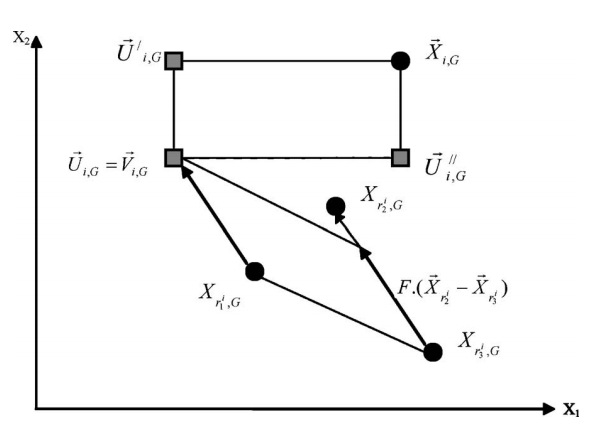
\includegraphics[scale = 0.5]{figures/crossover.png}
    \caption{Different possible trial vector formed due to Uniform/Binomial crossover between mutant vector and target vector in 2-D design space\cite{storn}.}
    \label{crossover}
\end{figure}

\begin{equation}
\mathbf{u}_{n,g}=\left\{\begin{array}{ll}{\mathbf{v}_{n,g}} & {\text { if rand }(0,1) \leq C R \text { or } r_{n}=d} \\ {\mathbf{x}_{n,g}} & {\text { otherwise }}\end{array}\right.
\label{cross-over}
\end{equation}
where $r_n$ is the uniformly distributed random integer in the interval [1, D], and $CR$ is the crossover probability. $CR = 1$ implies there is no diversity, meaning the parent individuals are not carried to the next generation. On the other hand, $CR = 0$ implies that all generated elements are the same as parent elements, so there is no evolution over generations.

\item \underline{Selection}: The trial individuals and target individuals are compared based on their function values. During the problem with the minimization case, an individual with minimum function value is retained. On the other hand, for maximization problems, an individual with a maximum function value is retained. Equation \ref{selection} represents the selection phase.
\begin{equation}
\mathbf{x}_{n}(t+1)=\left\{\begin{array}{ll}{\mathbf{u}_{n}} & {\text { if } f\left(\mathbf{u}_{n}\right) \leq f\left(\mathbf{x}_{n}(t)\right)} \\ {\mathbf{x}_{n}(t)} & {\text { otherwise }}\end{array}\right.
\label{selection}
\end{equation}

\item \underline{Stopping condition}: The optimization can have single or multiple stopping conditions, like the maximum number of function evaluations, epsilon value, to name a few. The author D.J.Poole used the maximum number of function evaluations ($FEs_{max}$) as the stopping condition for all the algorithms.
\end{enumerate}

The algorithm \ref{DE algorithm} depicts the pseudo-code for the DE algorithm.
\begin{algorithm}[!ht]
\SetAlgoNoLine
 Randomly initialise individuals and calculate objective\\
 \While{\text { $FEs <FEs_{max}$ }}
 {
  \For{$n=1 \rightarrow N$}
  {
  Perform mutation: equation \ref{best_mutation}\\
  Perform binomial crossover: equation \ref{cross-over}\\
  Calculate objective and constraints of trial vector
  }
  \For{$n=1 \rightarrow N$}{
 Update $n$-th target vector: equation \ref{selection}
 }
 }
 \caption{DE algorithm}
 \label{DE algorithm}
\end{algorithm}

In the next section, details about mutation strategies are explained. 

\section{DE Strategies}
In the DE algorithm, there are different variants for the mutation stage. Some of these are mentioned in the upcoming subsections \cite{chi}.

\subsection{DE/rand/1}
In this strategy, the mutation stage is carried out by taking single pair of the weighted difference. The individuals involved are randomly selected from the populations, Further, the weighted difference is added to base individual resulting in target vector as shown in equation \ref{DE-rand-1}.
\begin{equation}
    \mathbf{v}_{n, g}=\mathbf{x}_{r_{1}, g}+F.\left(\mathbf{x}_{r_{2}, g}-\mathbf{x}_{r_{3}, g}\right)
    \label{DE-rand-1}
\end{equation}

\subsection{DE/best/1}
This method work the same way as DE/rand/1 strategy, except that it generates the individual base vector $x_{b}$ as in equation \ref{DE-best-1}.
\begin{equation}
    \mathbf{v}_{n, g}=\mathbf{x}_{b, g-1}+F.\left(\mathbf{x}_{r_{1}, g}-\mathbf{x}_{r_{2}, g}\right)
    \label{DE-best-1}
\end{equation}
where,
$$
b=\underset{i \in\{1, \ldots, N\}}{\arg \min } f\left(\mathbf{x}_{i, g-1}\right)
$$

\subsection{DE/best/2}
This strategy involve evaluating the mutant vector with two weighted ($F_1, F_2$) differences of vectors which are picked randomly from the population size \(N\), and added to base vector (best) \(x_b\). Equation \ref{DE-best-2} represents the same.
\begin{equation}
  \mathbf{v}_{n, g}=\mathbf{x}_{b, g-1}
+F_{1}.\left(\mathbf{x}_{r_{1}, g}-\mathbf{x}_{r_{2}, g}\right)
+F_{2}.\left(\mathbf{x}_{r_{3}, g}-\mathbf{x}_{r_{4}, g}\right)
\label{DE-best-2}
\end{equation}
where,
$$
b=\underset{i \in\{1, \ldots, N\}}{\arg \min } f\left(\mathbf{x}_{i, g}\right)
$$

\subsection{DE/current to best/2}
In this strategy, one of the two weighted differences will take place between the best vector and the vector index for which perturbation is carried out. Equation \ref{DE-ctob-2} depicts the above strategy. 
$$\mathbf{v}_{n}=\mathbf{x}_{b}(t)
+F_{1}\left(\mathbf{x}_{r_{1}}(t)-\mathbf{x}_{r_{2}}(t)\right)
+F_{2}\left(\mathbf{x}_{b}(t)-\mathbf{x}_{r_n}(t)\right)$$
where,
$$
b=\underset{i \in\{1, \ldots, N\}}{\arg \min } f\left(\mathbf{x}_{i}\right)
$$

\subsection{DE/rand/2}
This strategy involve two weighted differences between individuals. These individuals are randomly selected in the given population. Equation \ref{DE-rand-2} represents the mutant vector generation using the DE/rand/2 strategy. 
$$\mathbf{v}_{n}=\mathbf{x}_{r_{1}}(t)
+F_{1}\left(\mathbf{x}_{r_{2}}(t)-\mathbf{x}_{r_{3}}(t)\right)
+F_{2}\left(\mathbf{x}_{r_{4}}(t)-\mathbf{x}_{r_{5}}(t)\right)$$
where, $r_1, r_2, r_3, r_4, r_5 \in [1, NP]$ and $\neq$ running index $i$. 


\subsection{Comparision between strategies}
The author H.Chi \cite{chi} mention that the strategies like \textit{DE/best/1}, \textit{DE/best/2} and \textit{DE/current to best/2} can improve the convergence rate of DE, and converge in the local optimal due to usage of the best vector. On the other hand, \textit{DE/rand/2} and \textit{DE/rand/1} relatively enhance the convergence rate of finding the global optimal but have slow convergence speed. Several test functions like Sphere function, Rosenbock's function, Step function, Quartic function, etc. are tested using the Niching algorithm, and results obtained coincide with the actual optimal values. Chapter \ref{results} highlights more on test function results.

\section{Constraint handling}
The feasibility rules published by Deb \cite{Daniel} assist in handling the constraints to the problems. The rules are as stated: when choosing between two
locations, if both locations are feasible, the one with the best fitness value wins. If a single location is feasible, then select the same. Otherwise, select the location with the least constraint violations. Mathematically, using domination operator, where, given two locations $x_a$ and $x_b$, $x_b$ dominates $x_a$ based on the conditions mentioned in equation \ref{feas}.
\begin{equation}
\mathbf{x}_{a} \prec \mathbf{x}_{b}
\Leftrightarrow\left\{
\begin{array}{ll}
{f\left(\mathbf{x}_{b}\right)<f\left(\mathbf{x}_{a}\right)} & {\text { and } \quad \phi\left(\mathbf{x}_{a}\right), \phi\left(\mathbf{x}_{b}\right)=0} \\
{\phi\left(\mathbf{x}_{b}\right)=0} & {\text { and } \quad \phi\left(\mathbf{x}_{a}\right)>0} \\
{\phi\left(\mathbf{x}_{b}\right)<\phi\left(\mathbf{x}_{a}\right)} & {\text { and } \quad \phi\left(\mathbf{x}_{a}\right), \phi\left(\mathbf{x}_{b}\right)>0}
\end{array}\right.
\label{feas}
\end{equation}

where $\phi$ is the constraint violation given by:

\begin{equation}
\phi (\mathbf{x})=\sum_{i=1}^{p} \max \left[0, g_{i}(\mathbf{x})\right]+\sum_{j=1}^{q}\left|h_{j}(\mathbf{x})\right|
\end{equation}

In DE, these feasibility rules are commonly used in the selection step to determine whether the trial vector should
replace the target vector. Hence at selection stage:

\begin{equation}
\mathbf{x}_{n}(t+1)=\left\{\begin{array}{ll}{\mathbf{u}_{n}} & {\text { if } \mathbf{x}_{n}(t) \prec \mathbf{u}_{n}} \\ {\mathbf{x}_{n}(t)} & {\text { otherwise }}\end{array}\right.
\label{selection_constraint}
\end{equation}

\section{Control variable}

There are a few parameters that decide the algorithm progress towards the optimal points. The $N$, $F$, and $CR$ are the essential parameters in the DE algorithm. D.J.Poole \cite{storn} states that it is not difficult to guess the range of values for these algorithms. According to the author, $N$ is to be between $5D$ and $10D$. A value of $F$ = 0.5 is usually the right choice. Furthermore, for $CR$ probability, a value of 0.1 would work fine. However, the higher the value of $CR$ faster will be the convergence. So it is always the better choice to test the algorithm with a $CR$ value of 0.9.

\section{Parallel and Sequential decomposition}
There are two ways to implement the algorithm, sequential flow, and parallel flow. Taking DE into consideration, the sequential form of DE constitutes the mutation, crossover, and selection phases in sequential order. For each population within a design space, all these phases are carried out in sequential order, as shown in figure [\ref{sequential_form_algo}]. However, this will result in an inefficient implementation. Instead, a parallel form of implementation can be followed. Here, the entire population is subjected to mutation, crossover, selection phases at once. Later, the comparison between the populations is carried out. 

The most expensive part of the aerodynamic optimization problem is objective function evaluation, which is CFD evaluation. In the case of solving the above problem, the parallel decomposition of algorithm wins over the sequential. Also, each of the population can be thread into single processing resulting in parallel computation of the CFD simulations. The pictorial representation of both parallel and sequential decomposition of the algorithm is shown in figure \ref{parallel_form_algo}.

\begin{figure}[!ht]
    \centering
    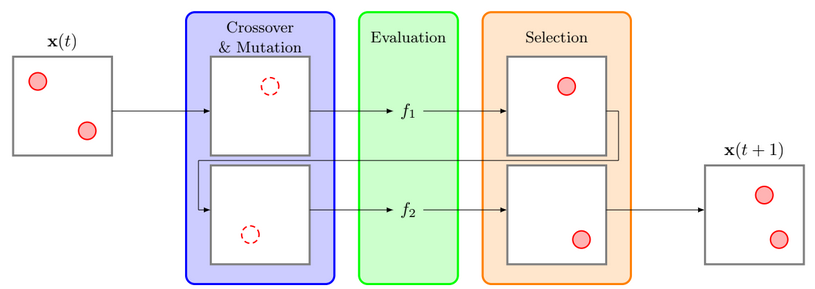
\includegraphics[scale = 0.5]{figures/sequential_form_DE.png}
    \caption{Sequential decomposition of algorithm\cite{Poole2}.}
    \label{sequential_form_algo}
\end{figure}

\begin{figure}[!ht]
    \centering
    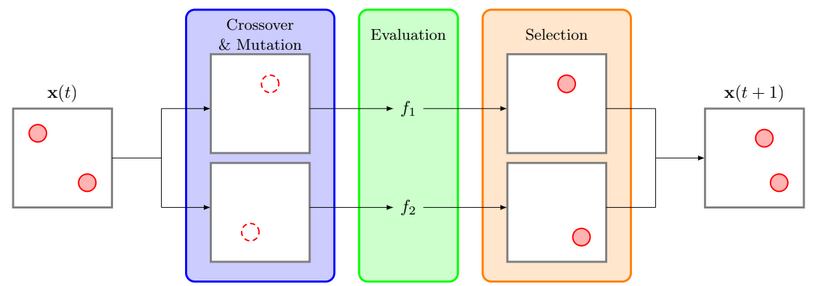
\includegraphics[scale = 0.5]{figures/parallel_form_DE.png}
    \caption{Parallel decomposition of algorithm\cite{Poole2}.}
    \label{parallel_form_algo}
\end{figure}

\section{Sequential niching algorithm}
As mentioned before, there are two ways to implement the DE algorithm. The upcoming subsections explain different sequential niching algorithms. Among these, few of the niching algorithms are recreated in Python and implemented on test functions like Ackley function, Rastrigin function, and Egg holder function. The result coincides with the one published by the author and is discussed in chapter \ref{results}. 

The algorithm involved in aerospace optimization generally follows the population crowding technique\cite{De_jong,thomsen}, fitness sharing\cite{michigan,thomsen,goldberg}, clearing\cite{petrowski}, speciation\cite{balazs,Li}, local neighborhoods\cite{vrahatis,vrahatis_1}, to name a few. Li $et$ $al$. present a full review of these properties\cite{li_1}. Following are few of the sequential niching algorithms which are implemented in Python and as follows \cite{Poole3}.
$$
\begin{array}{l}
{\bullet \text { Feasible DE }(\mathrm{fDE}), \text { which is based on canonical DE }} \\ 
{\bullet \text { Feasible DE using nrandl mutation (fNRAND1)}}\\
{\bullet \text { Feasible DE using inrand } 1 / r \text { (nearest neighbour with ring network) mutation (fINRAND1)}} \\
{\bullet \text { Feasible crowding DE (fCDE), which is based on the CDE algorithm }} \\
{\bullet \text { Feasible neighbourhood-based CDE (fNCDE), which is based on the NCDE algorithm  }} \\ {\bullet \text { Feasible species-based DE (fSDE), which is based on the SDE algorithm }} \\
{\bullet \text { Feasible neighbourhood-based SDE (fNSDE), which is based on the NSDE algorithm }} \\ {\bullet \text { Feasible fitness-sharing DE (fSHDE), which is based on the SHDE algorithm }}
\end{array}
$$
\subsection{fDE}
In this algorithm \ref{fDE algorithm}, the selection stage is modified as stated by Deb and Saha \cite{Deb}, which uses equation \ref{selection_constraint}. Additionally, the mutation stage follows $rand/1/bin$ strategy. Algorithm \ref{fDE algorithm} represents the same.
\begin{algorithm}[!ht]
\SetAlgoNoLine
 Randomly initialise individuals and calculate objective\\
 \While{\text { $FEs <FEs_{max}$ }}
 {
  \For{$n=1 \rightarrow N$}
  {
  Perform rand/1 mutation: equation \ref{best_mutation}\\
  Perform binomial crossover: equation \ref{cross-over}\\
  Calculate objective and constraints of trial vector
  }
  \For{$n=1 \rightarrow N$}{
 Update $n$-th target vector: equation \ref{selection_constraint}
 }
 }
 \caption{fDE algorithm}
 \label{fDE algorithm}
\end{algorithm}

\subsection{fNRAND1}
In the algorithm \ref{fNRAND1 algorithm}, mutation stage is modified by taking the target vector of the \(n\)-th individual's nearest neighbour $x_{{NN}_n}$ as the base vector. The selection stage uses equation [\ref{selection_constraint}] for feasibility check. Equation \ref{fNRNAD1_equation} represents the mutant vector. 
\begin{equation}
\mathbf{v}_{n, g}=\mathbf{x}_{N N_{n, g}}+F.\left(\mathbf{x}_{r_{1}, g}-\mathbf{x}_{r_{2}, g}\right)
\label{fNRNAD1_equation}
\end{equation}
where,
$$N N_{n, g}=\underset{i \in\{1, \ldots, N\}, i \neq n} {\arg \min} \left\|\mathbf{x}_{n, g}-\mathbf{x}_{i, g}\right\|_{2}$$

\begin{algorithm}[!ht]
\SetAlgoNoLine
 Randomly initialise individuals and calculate objective\\
 \While{\text { $FEs <FEs_{max}$ }}
 {
  \For{$n=1 \rightarrow N$}
  {
  Find the nearest neighbour to $x_n$\\
  Perform nrand/1 mutation: equation \ref{fNRNAD1_equation}\\
  Perform binomial crossover: equation \ref{cross-over}\\
  Calculate objective and constraints of trial vector
  }
  \For{$n=1 \rightarrow N$}{
 Update $n$-th target vector: equation \ref{selection_constraint}
 }
 }
 \caption{fNRAND1 algorithm}
 \label{fNRAND1 algorithm}
\end{algorithm}

\subsection{fINRAND1}
The fINRAND1 algorithm \ref{fINRAND1 algorithm} works similarly to that of the fINRAND1 algorithm. However, in the mutation stage, the algorithm uses the target vector of the \(n\)-th individual’s nearest neighbor within its local neighborhood, $x_{INN_n}$, as the base vectors. Since it uses an index-based ring neighborhood, this algorithm reduces the computational complexity against the fNRAND1 algorithm. Equation \ref{fINRAND1_equation} represents the same.
\begin{equation}
\mathbf{v}_{n, g}=\mathbf{x}_{I N N_{n, g}}+F.\left(\mathbf{x}_{r_{1}, g}-\mathbf{x}_{r_{2}, g}\right)
\label{fINRAND1_equation}
\end{equation}
where,

$$
I N N_{n, g}=\left\{
\begin{array}{ll}
{\underset{i \in\{N, 2\}}{\arg \min} \left\|\mathbf{x}_{n, g}-\mathbf{x}_{i, g}\right\|_{2}} & {\text { if } n=1} \\
{\underset{i \in\{N-1,1\}}{\arg \min}\left\|\mathbf{x}_{n, g}-\mathbf{x}_{i, g}\right\|_{2}} & {\text { if } n=N} \\
{\underset{i \in\{n-1, n+1\}}{\arg \min}\left\|\mathbf{x}_{n, g}-\mathbf{x}_{i, g}\right\|_{2}} & {\text { otherwise }}
\end{array}
\right.
$$
In the selection stage, equation \ref{selection_constraint} is used as feasibility criteria.
\begin{algorithm}[!ht]
\SetAlgoNoLine
 Randomly initialise individuals and calculate objective\\
 \While{\text { $FEs <FEs_{max}$ }}
 {
  \For{$n=1 \rightarrow N$}
  {
  Find the nearest neighbour to $x_n$ in ring neighbourhood\\
  Perform inrand/1 mutation: equation \ref{fINRAND1_equation}\\
  Perform binomial crossover: equation \ref{cross-over}\\
  Calculate objective and constraints of trial vector
  }
  \For{$n=1 \rightarrow N$}{
 Update $n$-th target vector: equation \ref{selection_constraint}
 }
 }
 \caption{fINRAND1 algorithm}
 \label{fINRAND1 algorithm}
\end{algorithm}

\subsection{fCDE}
This algorithm \ref{fDE algorithm} uses the standard CDE algorithm but with feasibility selection rules in the selection phase. In the CDE algorithm, the nearest individual $ {x}_{u_{n}} $ to the trial vector is found. The nearest individual replaces the target vector, which is determined using feasibility rules, as stated in equation \ref{feas}.

\begin{equation}
\mathbf{x}_{u_{n}}(t+1)=\left\{\begin{array}{ll}{\mathbf{u}_{n}} & {\text { if } \mathbf{x}_{u_{n}}(t) \prec \mathbf{u}_{n}} \\ {\mathbf{x}_{u_{n}}(t)} & {\text { otherwise }}\end{array}\right.
\label{fCDE-equation}
\end{equation}
\begin{algorithm}
\SetAlgoNoLine
 Randomly initialise individuals and calculate objective\\
 \While{\text { $FEs <FEs_{max}$ }}
 {
  \For{$n=1 \rightarrow N$}
  {
  Perform rand/1 mutation: equation \ref{best_mutation}\\
  Perform binomial crossover: equation \ref{cross-over}\\
  Calculate objective and constraints of trial vector
  }
  \For{$n=1 \rightarrow N$}{
  Find the closest individual to \textbf{$u_n$}\\
 Update closest individual: equation \ref{fCDE-equation}
 }
 }
 \caption{fCDE algorithm}
 \label{fCDE algorithm}
\end{algorithm}

\subsection{fNCDE}
The fNCDE algorithm \ref{fNCDE algorithm} follows the neighborhood search method. In this algorithm, the trial vector is generated from $m$ nearest individuals to the $n$-th individual, in the design space. While performing mutation, all three vectors are derived from the $m$ nearest neighbors. Further steps are the same as normal crowding DE.
\begin{algorithm}[!ht]
\SetAlgoNoLine
 Randomly initialise individuals and calculate objective\\
 \While{\text { $FEs <FEs_{max}$ }}
 {
  \For{$n=1 \rightarrow N$}
  {
  Find the nearest $m$ individuals to $x_n$\\
  Perform rand/1 mutation using the nearest $m$ individuals\\
  Perform binomial crossover: equation \ref{cross-over}\\
  Calculate objective and constraints of trial vector
  }
  \For{$n=1 \rightarrow N$}{
  Find the closest individual to \textbf{$u_n$} in the entire population\\
 Update closest individual: equation \ref{fCDE-equation}
 }
 }
 \caption{fNCDE algorithm}
 \label{fNCDE algorithm}
\end{algorithm}

\subsection{fSDE}
As compared to the above algorithms, the fSDE algorithm is considered to be the most time-consuming in terms of implementation and function evaluation. In this algorithm, initially, the population needs to sort in the ascending order satisfying the feasibility rules. If the individual satisfies the feasibility rules, then they are sorted based on the fitness values. However, any individuals violating the feasibility rules; they will be sorted in ascending order based on the constraint violations. Altogether both the populations are represented under the same variable name. The list is sorted from entire populations with the most feasibility individual at first in the list, and the individual violating at high degree will be placed at the last in the list. Furthermore, species are determined based on the distance from the species seed.  

Additionally, the species radius $\sigma$ is set by the user. Suppose the species has less than m (user-defined) individuals. In that case, the extra individuals are randomly added to the species radius to make all equal sets of individuals around every species. During $DE/rand/1$ mutation, $r1$, $r2$, and $r3$ are uniformly distributed random integers selected from $m$ individuals of the species representing the $n$-th individual. Since the population has been increased, only the first $N$ fittest individuals are kept for the next iteration, determined by feasibility rules. The overall algorithm is outlined in algorithm \ref{fSDE algorithm}.
\begin{algorithm}[!htbp]
\SetAlgoNoLine
 Randomly initialise individuals and calculate objective\\
 \While{\text { $FEs <FEs_{max}$ }}
 {
 Generate species: algorithm \ref{species generation algo} \\
  \For{$n=1 \rightarrow N$}
  {
  Perform rand/1 mutation using individuals within the species of $n$-th individual \\
  Perform binomial crossover: equation \ref{cross-over}\\
  Calculate objective and constraints of trial vector\\
  If trial fitness is same as its species seed, then randomly generate new trial vector
  }
  \For{$n=1 \rightarrow N$}{
 Update $n$-th target vector: equation \ref{selection_constraint}
 }
 Compare individuals using feasibility rules and keep $N$ fittest individuals
 }
 \caption{fSDE algorithm}
 \label{fSDE algorithm}
\end{algorithm}

\begin{algorithm}[!htbp]
\SetAlgoNoLine
 Sort individuals based on feasibility rules\\
 Sorted individuals are assigned to possible candidate solutions\\
 First species seed is best candidate solution-remove that solution from candidates\\
\For{$n=1 \rightarrow N$}
  {
  \For{$s=1 \rightarrow $ number of species}
  {
  \uIf {$n$-th candidate entry is not empty and is less than $r_s$ away from $s$-th seed} 
  {
  Solution is not a new seed\\
  Note solution is in $s$-th species\\
  }
  }
  \uIf {$n$-th candidate entry is new seed} 
  {
  Increment number of species \\
  Store $n$-th candidate solution as seed and remove from list of candidates\\
  }

  }
  \For{s = 1 $\rightarrow$  \text{number of species}}{
 If the $s$-th species has less that $m$ individuals, randomly generate new individuals within radius of species seed
 }
 
 \caption{fSDE species generation algorithm}
 \label{species generation algo}
\end{algorithm}

\section{Parallel niching algorithm}
The parallel niching algorithm involves performing mutation to all individuals, then subjecting all individuals to cross-over phase, further to selection phases. All these phases are performed in separate loops. Furthermore, it results in separating the workload and performed in different threads of the CPU. The bottleneck in the wing shape optimization is objective function evaluation (CFD simulation). All populations can be subjected to the individual thread for CFD simulation to obtain better performance and time-efficient. For example, the fNRAND1 algorithm with parallel decomposition is highlighted in the algorithm \ref{fNRAND1_parallel_algorithm}.
\begin{algorithm}
\SetAlgoNoLine
 Randomly initialise individuals and calculate objective\\
 \While{\text { $FEs <FEs_{max}$ }}
 {
  \For{$n=1 \rightarrow N$}
  {
  Find the nearest neighbour to $x_n$\\
  Perform nrand/1 mutation: equation \ref{fNRNAD1_equation}\\
  Perform binomial crossover: equation \ref{cross-over}\\
  }
  \For{$n=1 \rightarrow N$}{
  \uIf{$n = procid$}
  {
  Objective of n-th trial vector
  }
  }
  \For{$n=1 \rightarrow N$}{
 Update $n$-th target vector: equation \ref{selection_constraint}
 }
 }
 \caption{Parallel decomposition of fNRAND1 algorithm\cite{Poole2}}
 \label{fNRAND1_parallel_algorithm}
\end{algorithm}

\section{Parameter Tuning}
From the literature review, a higher number of generations will result in tremendous computational resources. The number of runs on each function set to be fifty for all the niching algorithms, while the population $N$ is suggested as $N=40 \sqrt{D. G}$, where $D$ is the dimension of problem, $G$ is maximum generation opted. Each niching algorithms perform better at a specific range of mutation factor and a crossover probability. The author D.J.Poole \cite{Poole3} suggested the values after considering all these factors and is mentioned in table \ref{niching_algo_parameters}.

\begin{table}[!ht]
\centering
\begin{tabular}{ccccccccc}
\hline
& {} & {} & {} &  {\text { Algorithm }} \\ 
\hline 
\text{Param} & \text {fCDE} & \text {fDE} & \text {fINRAND}1  & \text {fNCDE} & \text { fNRAND1} & \text {fNSDE} & \text {fSDE} & \text {fSHDE} \\ 
\hline 
C R & {0.1} & {0.1} & {0.9} & {0.9} & {0.9} & {0.1} & {0.9} & {0.1} \\ {F} & {0.1} & {0.9} & {0.9} & {0.9} & {0.9} & {0.9} & {0.9} & {0.1} \\ 
${\sigma}$ & {} & {} & {} & {} & {} & {} & {  10 \%} & {  0.1 \%} \\ 
{m} & {} & {} & {} & {10} & {} & {10} & {20} \\ 
\hline
\end{tabular}
\label{niching_algo_parameters}
\caption{Parameter tuned for different niching algorithms\cite{Poole3}.}
\end{table}

\section{Conclusion}

The two neighborhood-based
algorithms (fNSDE and fNCDE) have the fastest overall convergence rates. However, fNSDE
has little difficulty finding all of the optima quickly, and the niches formed appear to be \textbf{unstable}. For example, fNSDE locates all of the optima rapidly and then cannot maintain these niches. However, for function F14 (\textit{modified Rastrigin function}), the majority of optima are located. However, the niches are unstable, resulting in global optima. On the other hand, fNCDE located optima at a slightly slower rate than fNSDE but is able to maintain stable niches. The average convergence speed of fDE is lower than fCDE, fINRAND1, fSDE and fSHDE, which demands for greater complexity as compared to fDE.

In terms of algorithmic development, fINRAND1 and fNRAND1 require the least effort to develop, with only a few extra lines of code added and no change in code logic. On comparing \textbf{fDE} and \textbf{fNRAND1}, the \textbf{fNRAND1 is superior} in terms of convergence speeds, peak ratios, and success rates. The fNRAND1 involves finding the nearest neighbor individual, increasing the algorithm complexity by up to $O(N^2)$ per iteration, compared to $O(N)$ for fDE.

The fDE inherently has difficulty maintaining stable niches and appears to converge to global optima or single optima. For function F14 (Himmelblau function), it appears that fDE has four optimal. However, with additional generations, all optimal points merge to a single point.

During higher functional evaluation, the comparison of PR (Peak Ratio) \cite{Poole3} points to three unique best-performing algorithms: \textbf{fCDE, fNCDE, and fNRAND1}. If the function evaluation is of lower quantity, the explicit winner is \textbf{fNSDE}. As discussed before, fNSDE is outstanding at creating niches. Higher the algorithm evolves, the greater are the chance of niches break down. The fNRAND1 is simple to implement, whereas its neighbor, fINRAND1, has an excellent overall performance. The more complex algorithm wins against, the fewer one. However, the trade-off in complexity is a call for an hour.

The results of the test function evaluation are mentioned in chapter \ref{results}. Furthermore, the respective test function equations will be appended in the appendix \ref{app_c}. 

\chapter{Parameterization of wing}     %chapter three
\begin{frame}[allowframebreaks]{\underline{Parameterization} -}
    \section{Parameterization}
    
\underline{Free Form Deformation technique :} FFD is a process by which shape to given geometry is achieved by manipulating the
location of control points. 
\begin{itemize}
\item It is easy to implement.
\item  More flexible while perturbating control points.
\end{itemize}
\vspace{1mm}
\underline{The 3D FFD equation:} 
  \begin{equation}
\mathbf{X}_{(u, t, s)}=\sum_{i=0}^{m} \sum_{j=0}^{n} \sum_{k=0}^{p} f_{i}^{m}(u) g_{j}^{n}(t) h_{k}^{p}(s) \mathbf{P}_{(i, j, k)}
\label{ffd_3d}
\end{equation}
where $\mathbf{P}_{(i, j, k)}$ is perturbed control points, $\mathbf{X}_{(u, t, s)}$ new coordinates of wing surface points, and Bernstein's polynomial $f_{i}^{m}(u)$ is defined as,
\begin{equation}
f_{i}^{m}(u)=\frac{(m) !}{(i) !(m-i) !} u^{i}(1-u)^{m-i}
\label{bernstein_poly}
\end{equation}

\begin{figure}
\parbox{0.49\linewidth}
{
\centering
 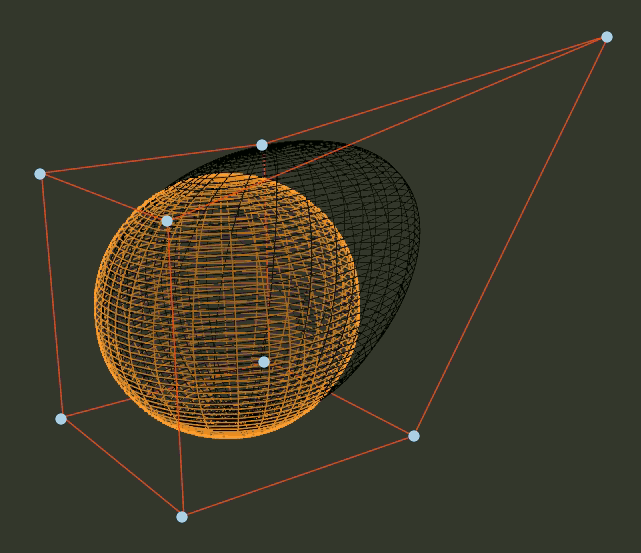
\includegraphics[scale = 0.15]{figures/sphere_ffd.png}
 \caption{Influence of the control point over the sphere body with $a^{(m,n,p)}$ as $2 \times 2 \times 2$ control points.}
 \label{sphere_ffd}
}
\parbox{0.47\linewidth}
{
\centering
   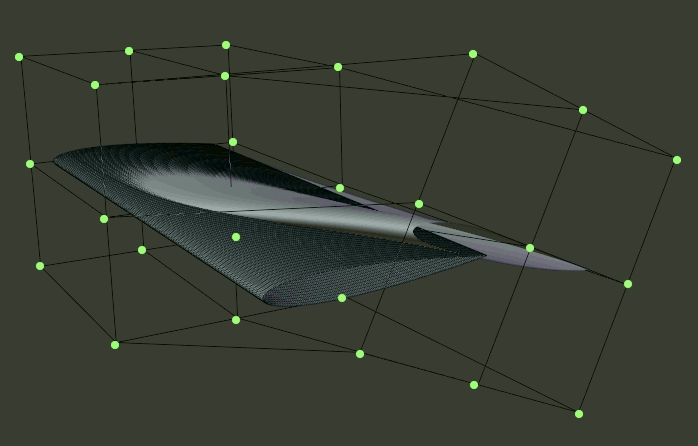
\includegraphics[scale = 0.15]{figures/ffd_wing.png}
  \caption{FFD of a wing shape, with the control points on the face of the wing-tip end are rotated and translated.}
  \label{wing_ffd}
}
\end{figure}
\begin{itemize}
    \item Figure \ref{sphere_ffd} represents the effect of control point perturbation over sphere.
    \item The effect of perturbation diminishes with distance from control point perturbed.
    \item Introducing more control points will provide better control over shape.
\end{itemize}

\begin{figure}
    \parbox{0.35\linewidth}
    {
    \centering
    \framebox{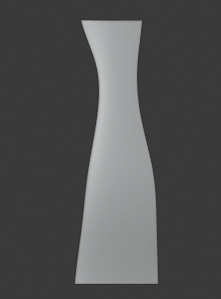
\includegraphics[scale=0.4]{figures/wing6_span.png}}
    \caption{Span view of wing 2.}
    \label{wing2_span}
    }
    \parbox{0.6\linewidth}
    {
    \centering
    \framebox{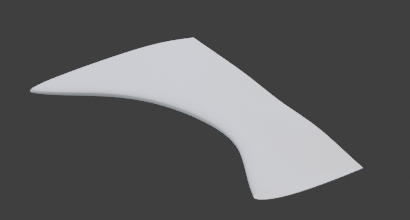
\includegraphics[scale = 0.4]{figures/wing2_iso.png}}
    \caption{Iso view of wing 1.}
    \label{wing1_iso}
    }
\end{figure}
\begin{itemize}
\item Figure \ref{wing2_span} and \ref{wing1_iso} illustrates the wings obtained with 60 control points.
\item With proper tuning of limits, it is possible to obtain twist, dihedral, taper characteristic to the wing.
\end{itemize}

\end{frame}

\chapter{Solver}                       % chapter four
\chapter{CFD Solver}
\label{solver}
\section{Background}
In a recent decade, the capability of computational analysis and optimization has made considerable improvement, which made many researchers rethink solutions to real-world problems. One such problem addressed here is the optimization of wing surface geometry. There requires several software packages and link them using some tools to address these problems. In the entire process of wing shape optimization, the bottleneck is found to be a CFD solution. More importance needs to be given to minimize the time taken by the solver. The SU2 solver is chosen based on its ease of availability and other constraint involved. The solver is initially tested on sample wing shape (NACA 0012 wing) for its reliability, and results seem positive. Also, the SU2 solver is open-source. Hence, more flexibility will be available to tweak the code. In this chapter, more emphasis is given to implement the SU2 solver and Pointwise (meshing software).

\section{Using meshing software}
sdsdds

\section{Using CFD solver}
sdsdsd
\section{Job submission}
sdsds

\chapter{Conclusion}                   % chapter five
\chapter{Result and Discussions}
\label{results}
Once all software packages are aligned under a single python script, the python script is fired into the HPC cluster. After covering a considerable amount of time, the results are extracted, and the post-processing is carried using Paraview. This chapter contains detailed information about the number of computational hours used, the CFD solver setup, optimized wings, and more importantly, the comments over the obtained results.

The objective function that is aimed is the drag coefficient minimization. Furthermore, the drag is made up of two parts. They are pressure drag and the induced drag. Since this work involves the inviscid solution, the drag represented here will be the induced drag alone. Equation \ref{induced_drag} represents the equation for induced drag evaluation \cite{Poole1}. 
\begin{equation}
C_{D_{i}}=\frac{C_{L}^{2}}{\pi A R}(1+\delta)
\label{induced_drag}
\end{equation}
where,\\
$$\delta=8\left(\frac{3 \pi}{2} \frac{C_{M_{x}}}{C_{L}}-1\right)^{2}$$

For the given problem (ADODG case 6) with aspect ratio 6, the theoretical minimum induced drag is found to be 25.5 counts (1 count = $10^{-3}$ drag units).

\section{Algorithm Assessment: Finding local minima for the test functions.}
The niching algorithm is initially tested on an analytical test function to assess their performance. Appendix \ref{app_c} contains the test functions that are analyzed. For example, consider the sphere function, as shown in equation \ref{Sphere function}.

\begin{equation}
f(\mathbf{x})=\sum_{i=1}^{d} x_{i}^{2}
\label{sphere_function}
\end{equation}

Further, the test function is subjected to constraints as mentioned in \cite{Poole3}. There exists four optima located at (1, 1), (-1, 1), (-1, -1), and (1, -1). Niching algorithm as mentioned in chapter \ref{niching} are implemented over this test function and the result are promising. Figure \ref{init_pop} illustrates the outcome of fINRAND1 niching algorithm over the given 2-D test function. 
\begin{figure}[!htbp]
\parbox{0.47\linewidth}
    {
    \centering
    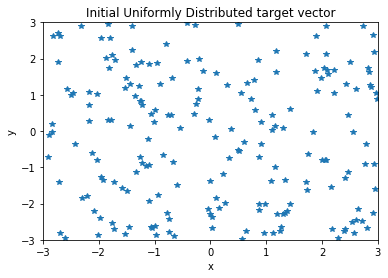
\includegraphics[scale = 0.5]{figures/initial_pop.png}
    \caption{Initial 200 population.}
    \label{init_pop}
    }
\parbox{0.47\linewidth}
    {
    \centering
    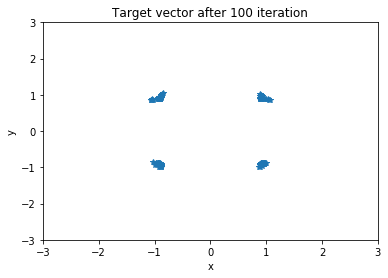
\includegraphics[scale = 0.5]{figures/final_target.png}
    \caption{Optimal points after 100 generations.}
    \label{target_points}
    }
\end{figure}

Overall, a population of 200 are used within the design space $x_1:(3, -3)$ and $x_2:(3, -3)$. A total of 100 generations are carried out to get an optimal solution. However, in the case of CFD simulation running for such higher generations seems impractical. A trade-off is required between the generations and the solutions obtained. This confirms that the algorithm is capable of identifying the local optima in a given design space.

\section{Computational power}
In the initial stage, the niching algorithms were tested in the workstation with Intel Xeon W-2155 @ 3.3 GHz, 20 CPU. However, the assigned workstation would not be sufficient to run the full-fledged optimizer. As a result, the entire work is executed in the HPC cluster containing 56 CPU with Intel Xeon E5-2690 @ 2.6 GHz. This work demands for 20 CPU of a given compute node and takes less than 180 minutes to complete a generation.

\section{Grid sensitivity analysis}
In the entire optimization process, the objective function evaluation (CFD simulation) is a bottleneck. With higher mesh points, more will be the computational cost. So it is very crucial to choose the mesh size, which is feasible for given computational power. A baseline wing with two mesh quality is generated. Table \ref{grid_sensitivity} provide additional details about the mesh quality.

\begin{table}[!htbp]
    \centering
    \begin{tabular}{|c|c|c|}\hline
        \textbf{Mesh quality} & \textbf{Surface mesh} & \textbf{Volume mesh} \\\hline
        Coarse  & 150 $\times$ 100 & 0.11m \\
        Fine  & 300 $\times$ 200 & 0.25m \\\hline
    \end{tabular}
    \caption{Grid sensitivity analysis}
    \label{grid_sensitivity}
\end{table}
The baseline wing with coarse mesh (150 along the chord, 100 along the span) would take less than 50 minutes (workstation) to complete the CFD run, whereas, the fine mesh takes about 120 minutes (workstation). Further, with additional lift coefficient constraint the fine mesh completed the CFD run in 180 minutes (workstation). This implies if the problem is set to run in parallel with each CPU assigned to one of the perturbed wings, after every 180 minutes, one optimization generation get completed. 
\begin{figure}[!htbp]
    \centering
    \framebox{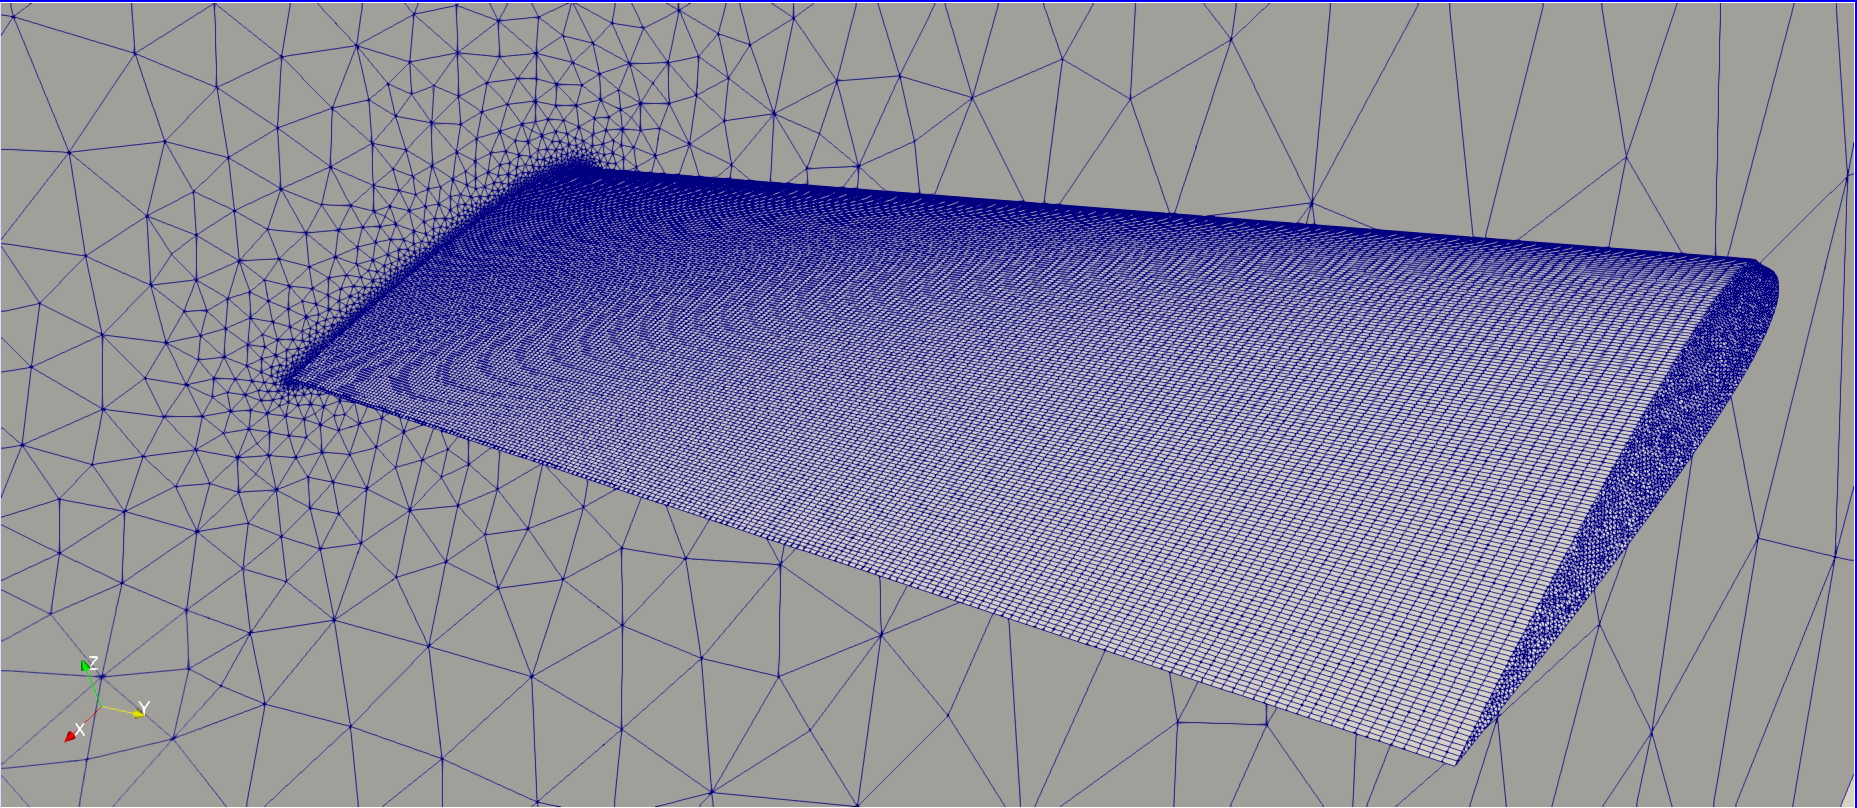
\includegraphics[scale = 0.22]{figures/fine_mesh_wing.png}}
    \caption{Fine mesh with 300 $\times$ 200 surface mesh points.}
    \label{fine_mesh}
\end{figure}

Figure \ref{fine_mesh} represents the fine mesh containing 0.25m mesh points with 300 $\times$ 200 mesh points over the wing surface. The distribution of mesh points at the symmetry surface is appropriate. Cell size is increasing from the wing surface towards the wall surfaces at a rate of 20\%.
\begin{figure}[!htbp]
    \centering
    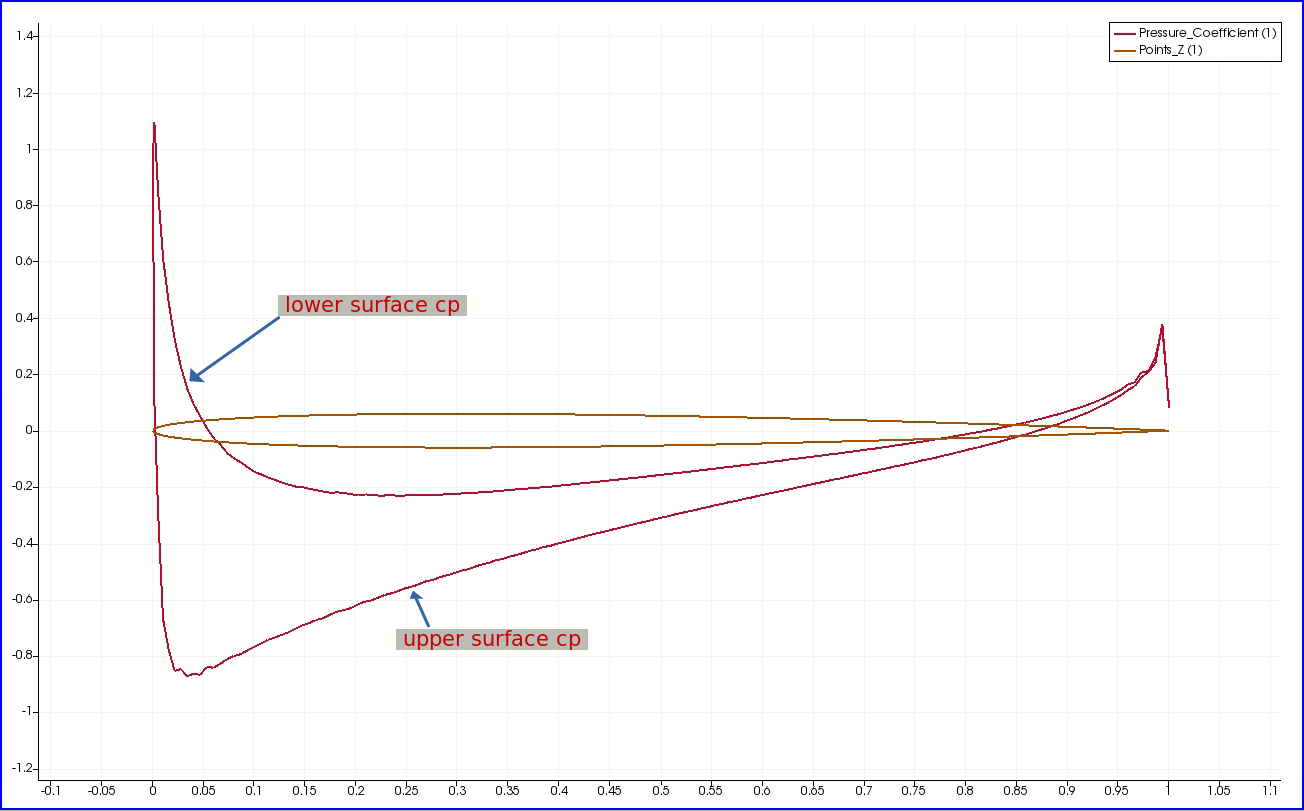
\includegraphics[scale = 0.3]{figures/cp_curve.png}
    \caption{Cp curve at root section of fine mesh (300 $\times$ 200).}
    \label{cp curve}
\end{figure}

Figure \ref{cp curve} represents the coefficient of pressure at the root section of the baseline wing for a fine mesh. The results of the cp curve meet the expected values. There is some disturbance in the Cp curve at the trailing edge. The reason for this is because the airfoil has a sharp trailing edge. The fine mesh appears appropriate to proceed with full optimization.

\section{Multimodality}
In this problem, the flow is subsonic and inviscid. The objective is to minimize the drag coefficient of $C_d$. The Mach number is 0.4. The lift coefficient of $C_l$ is constrained to 0.2625. The angle of attack is varied between -3$^0$ and +6$^0$. The angle of attack is a design variable which is optimized using CFD solver. The root bending moment is constrained to be $\leq$ 0.1039. Geometry is parameterized using the FFD box with 5 points along chord direction, 2 points along the thickness direction, and 6 points along the span direction, resulting in 60 control points. Each perturbed wing can vary in span direction between 2.7 units and 3.3 units. Due to FFD box control points perturbation, the perturbed wing will possess the twist and sweep angles. Each of the control points is perturbed such that it always results in feasible wings. More details on FFD control point perturbation is mentioned in chapter \ref{methodology}.

The first 20 initial geometries (population) generated by the random selection of point within the PCA selected design space is shown in figure \ref{initial_population}. These population cover all the design space like dihedral, taper wings, sweep backward/forward, winglet up/down, and span long/short.

\begin{figure}[!htbp]
    \centering
    \framebox{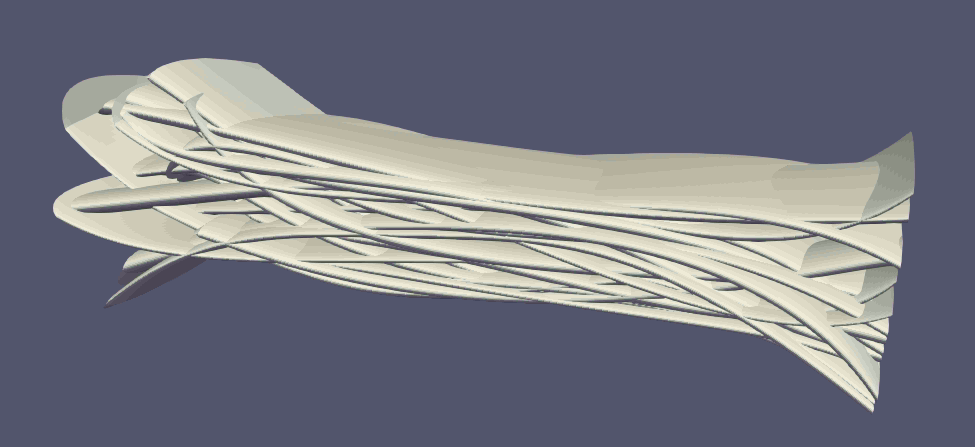
\includegraphics[width=0.95\textwidth, height=70mm]{figures/initial_population.png}}
    \caption{Initial 20 populations.}
    \label{initial_population}
\end{figure}

\begin{figure}[!htbp]
    \centering
    \framebox{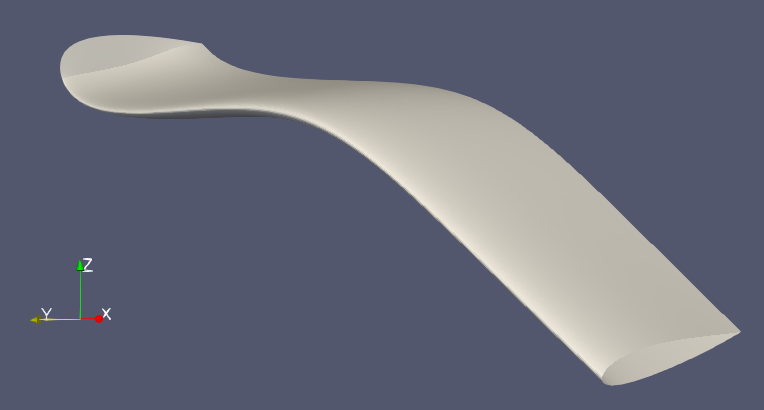
\includegraphics[width=0.95\textwidth, height=70mm]{figures/isoview_localwing_1.png}}
    \caption{Isometric view of local optima 1.}
    \label{isoview_localoptima_1}
\end{figure}

Since the flow is subsonic and inviscid, only the induced drag is present. The baseline (NACA 0012) geometry has $C_d$ of 5.08 $\times$ $10^{-2}$, with $C_l$ constraint satisfied by adjusting the angle of attack. After 1000 objective function evaluation, the first local optima was found to possess the $C_d$ value of 1.12 $\times 10^{-2}$. Figure \ref{isoview_localoptima_1} and \ref{frontview_localoptima_1} illustrates the isometric and leading-edge view of local optima 1 respectively.

\begin{figure}[!htbp]
    \centering
    \framebox{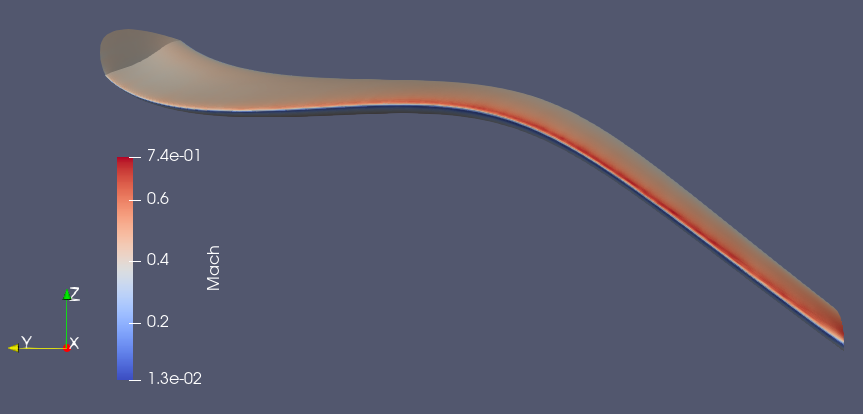
\includegraphics[width=0.95\textwidth, height=70mm]{figures/frontview_localwing_1.png}}
    \caption{Leading edge view of local optima 1.}
    \label{frontview_localoptima_1}
\end{figure}


Figure \ref{cp_curve in span direction} represents the Cp distribution for local optima 1 at three sections, that is, root section, midsection, and tip section. At root section, near the leading edge, there is a sharp decline in Cp value in the upper surface. The reason for this is incorrect volume mesh generation around the leading edge. A similar explanation can be provided for trailing edge Cp disturbance. The airfoil is twisted by small value and lift by a unit in the midsection of the span. At the tip section, the results got disrupted entirely. The airfoil is highly perturbed, resulting in negative lift.

After further analysis, it was found that the glyph script, that was designed to automate the volume mesh generation is incorrect. The script could not generate enough mesh points to get correct CFD results. No conclusion can be drawn from incorrect CFD solution. Due to insufficient time, the glyph script could not be corrected. However, assuming that the CFD results are correct, table \ref{optimal shape} represents local optima with additional details. More on these optima is covered in the upcoming section.

\begin{figure}[!htbp]
  \parbox{0.47\linewidth}{
    \centering
    \framebox{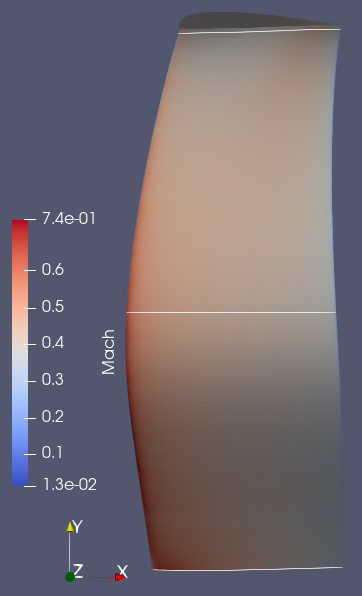
\includegraphics[width=0.9\linewidth, height=150mm]{figures/local_wing_1_span.png}}
    }
  \parbox{0.47\linewidth}{
    \centering
    \framebox{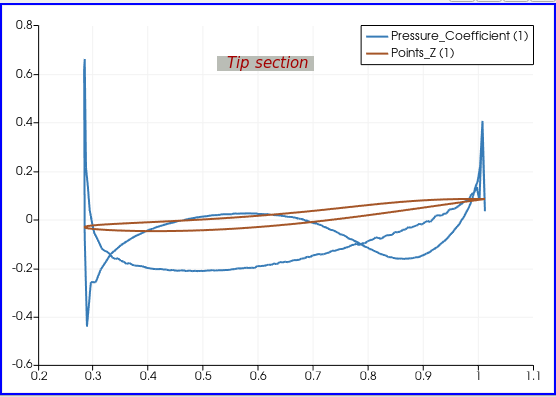
\includegraphics[scale=0.35]{figures/local_wing_1_tip_section.png}}
    \framebox{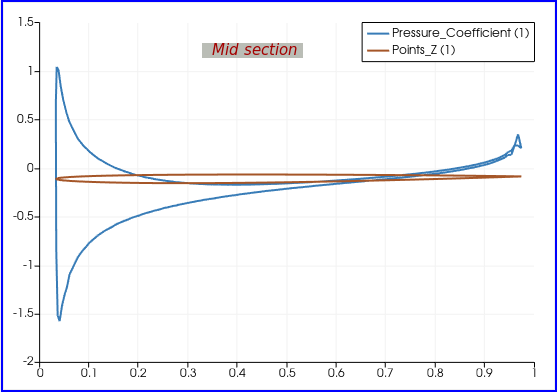
\includegraphics[scale=0.35]{figures/local_wing_1_mid_section.png}}
    \framebox{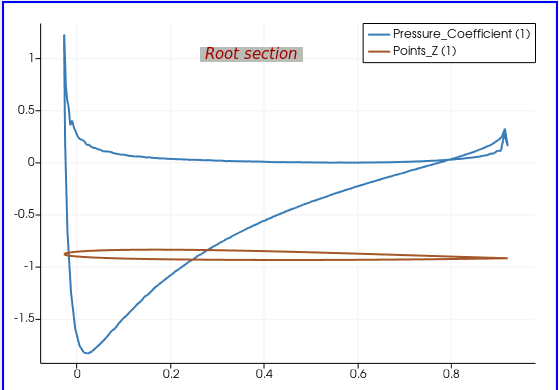
\includegraphics[scale=0.35]{figures/local_wing_1_root_section.png}}
    }
    \caption{Cp distribution at various sections in local optima 1 along span directions.}
    \label{cp_curve in span direction}
\end{figure}

\begin{table}[!htbp]
    \centering
    \begin{tabular}{|c|c|c|c|c|c|c|}\hline
          & $C_l$ & $C_d$ & $C_{M_x}$ & $AoA$ & Span & Obj.diff \\\hline
        local optima 1 & 0.2625 & 0.01120   & 0.1038 & 5.535$^0$ & 2.779 & 0.0\%\\
        local optima 2 & 0.2625 & 0.01203   & 0.1005 & 3.213$^0$ & 2.918 & 7.4\%\\
        local optima 3 & 0.2625 & 0.01204   & 0.1028 & 1.972$^0$ & 2.726 & 7.5\%\\
        local optima 4 & 0.2625 & 0.01215   & 0.998  & 2.774$^0$ & 3.291 & 8.4\%\\ \hline
    \end{tabular}
    \caption{$C_d$ values for various local optima.}
    \label{optimal shape}
\end{table}

\section{Discussion}

After a detailed examination of all steps, it is noticed that the wing parameterization, the FFD box implementation, the PCA implementation, and niching algorithm implementation is working correctly. The sole issue for incorrect results was inadequate volume mesh points. To reduce the computational cost, the number of mesh points is kept on the lower side (0.25m). With the same number of mesh points, the grid sensitivity analysis is carried out for baseline geometry, and the results (cp curve) seems acceptable. 

Following this, the same glyph script, which is meant for volume mesh generation, is used to generate the volume mesh for perturbed wings. However, at the end of full optimization, it was found that the grid resolution and grid clustering algorithm was not adequate, which resulted in erroneous flow-field. Also, at some sections in the optimal wings, inverted airfoils are generated. The cp curve shows inappropriate behaviour at those sections and is propagated through all sections of the given wing. Figure \ref{cp_curve in span direction} depicts the same.

The present work aimed to identify the existence of multimodality in a given design space. However, due to the present situation, COVID-19 pandemic, the work is partially completed. Also, glyph script can not be corrected remotely.

\begin{figure}[!htbp]
    \centering
    \framebox{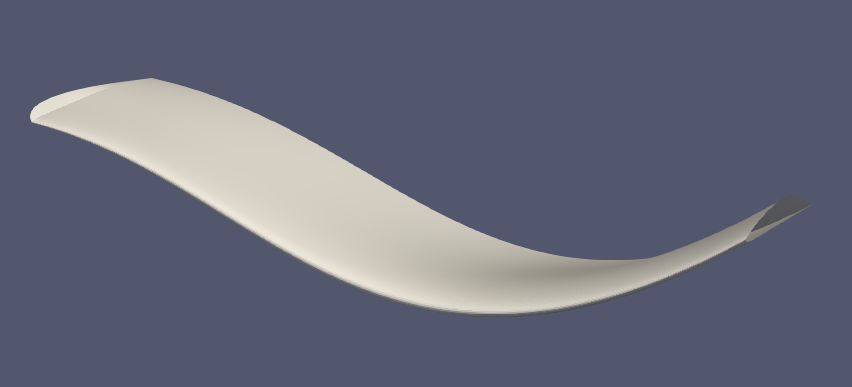
\includegraphics[width = 0.95\textwidth, height = 60mm]{figures/wing_13_iso.png}}
    \caption{Local optima 2}
    \label{local optima 2}
\end{figure}

\begin{figure}[!htbp]
    \centering
    \framebox{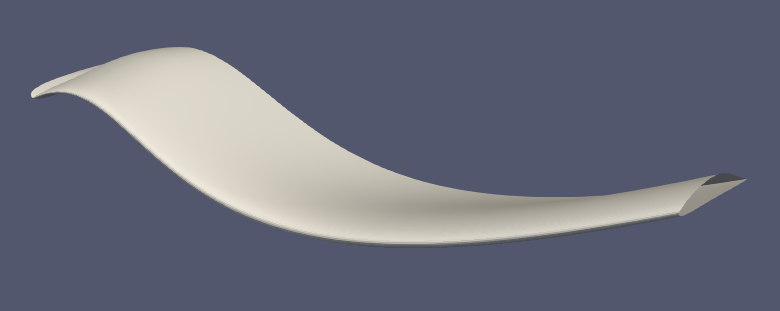
\includegraphics[width = 0.95\textwidth, height = 60mm]{figures/wing_20_iso.png}}
    \caption{Local optima 3}
    \label{local optima 3}
\end{figure}

\begin{figure}
    \centering
    \framebox{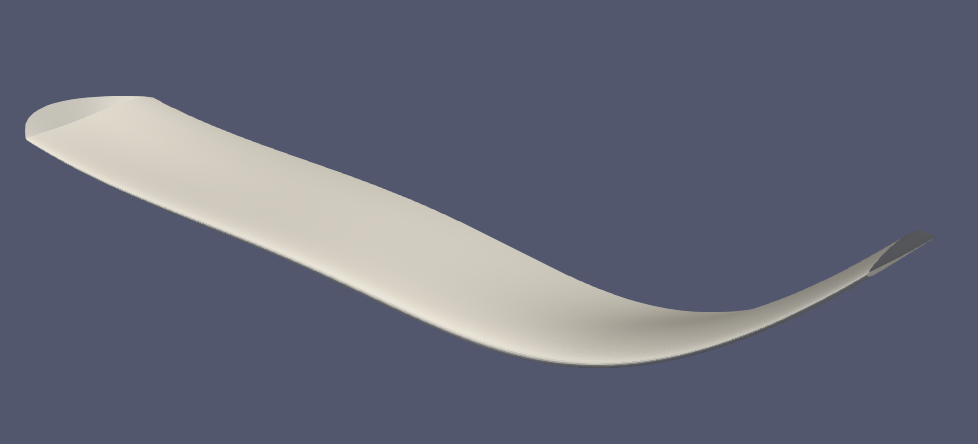
\includegraphics[width = 0.95\textwidth, height = 60mm]{figures/wing_14_iso.png}}
    \caption{Local optima 4}
    \label{local optima 4}
\end{figure}

Assuming that the CFD solution is correct, figure \ref{local optima 2} to \ref{local optima 4} represents the local optima in the increasing order of their objective values. Local optima 2 (figure \ref{local optima 2}) show an anhedral behaviour at the root section and dihedral at the wing tip section. There exists a smooth transition between an anhedral and the dihedral wing sections. Local optima 3 (figure \ref{local optima 3}) contain the waveform at the wing-tip section. Furthermore, a small leading-edge sweepback angle is observed in the root section. Local optima 4 (figure \ref{local optima 4}) reach the upper limit of span (3.3 units). 

The objective function of these optima varies by less than 9\%. As compared to results in Chernukhin \cite{oleg:phd}, the relative difference of objective function is on the higher side. The mesh size that is generated by the glyph script is five times lower. Furthermore, the objective function is found to be ten times higher.

\section{Future work}
This work addresses some of the issues with regards to the implementation of the FFD box, choice of design space, the dimension reduction techniques, winglet creations, and others. There exists some more critical question that needs to be addressed. As mentioned, the glyph script failed to reach the expectation. Further work is necessary to improve the performance of glyph script. Also, the choice of design space needs to be examined.

Further, niching algorithms requires computationally expensive CFD simulation. Reducing the number of CFD runs will significantly reduce the time taken for full optimization. As mentioned by Chernukhin \cite{oleg:phd}, performing the optimization under viscous flowfield will decrease the number of optima. Once all the above objectives are addressed, the work can further extended to viscous flowfield. 


%\chapter{Constraint}
%\chapter{constraint}
This chapter consists of the constraint which are being implemented in various papers and are listed below. 

\section{\underline{D.W.Zingg}}

The optimization problem is to minimize the drag coefficient ($C_D$), which is the function of \textbf{v} and \textbf{q}, where \textbf{v} is the vector of geometric DV, and \textbf{q} are the flow variables.

\subsection{Design Variables}
\begin{itemize}
\item The root of the wing is fixed in all three dimensions - \textbf{though sectional control and chord changes are permitted.}
\item Either an AoA or root twist should be a design variable.
\item At points other than root all DV are permitted to get perturbed : twist, taper, sectional, sweep, span and dihedral subjected to linear or non-linear constraint.
\end{itemize}

\subsection{Constraints}

\begin{itemize}
\item C$_L$ must be 0.375.
\item Projected are must be constrained to initial value 3.06 units.
\item Total volume should be at least 0.245 sq. units, which includes both body and wing tip cap.
\item Root Bending Moment constraint $C_{M_x}$ = ???.
\item Twist is limited to $\pm 2.0 $ degrees.
\item Chord can vary between 0.45 to 1.550.
\item Cross-sectional thickness may not vary by more than $\pm$ 50$\%$.
\item Span may vary between 2.46 to 3.67.
\item Sweep is achieved by shearing the wing while maintaining the span such that the quarter chord location at the tip is no more than \textbf{$\pm$ 1 chord length} from its original position.
\item \textbf{Dihedral may not take a value such that the vertical position of the quarter chord lies more than 0.45 chord lengths above or below its initial position.}
\end{itemize}

\section{\underline{Chernukhin}}
\subsection{Geometry}
Baseline Geometry is NACA0012 with sharp trailing edge.
\begin{itemize}
\item Semi span = 3.06 units.
\item Geometry is rectangular and planar, with no twist, taper, sweep or dihedral also with \textbf{pinched wingtip cap} over the last 0.06 units of span.\cite{oleg} 
\end{itemize}
\subsection{Constraint}
Constraints implemented by \textbf{Chernukhin} are as follows:

The paper is focused on \textbf{optimizing of cross sections} of wing by allowing the interior points to move only in vertical direction. 
\begin{itemize}
\item $C_L$ = 0.2625
\item Volume = at least 6.57 $\times$ 10$^{-2}$, which is the volume of the original wing.
\item Projected area (Semi-span) is constrained to 4/3.
\item AoA can vary between -3 to +6 deg.
\item \textbf{The control point at the trailing edge can have a maximum span wise extent of 2.4, maximum sweep back to 1.00, from the original value of 0.33, vertical bounds  are -0.3 and 0.3.}
\item Each sections are allowed to twist and change its shape.
\item Both leading and trailing edges can be curved.
\end{itemize}

Local optimum 2 is better than local optimum 7. (ref table 2 from paper). 

\section{\underline{D.J.Poole}}
\subsection{Constriants}
In the Previous two papers the DV are the position of control points. But in this paper the DV are the geometric parameters like chord, thickness, etc., of the wing. And is mathematically represented by,

$$  
\begin{aligned} 
{0.2625-C_{L} \leq 0} \implies \text{Coefficient of Lift} \\ 
{C_{M_{x}}-0.1069 \leq 0} \implies \text{Root bending moment}\\
{V_{initial}-V \leq 0} \implies \text{Volume}\\ 
{2.46 \leq s \leq 3.67} \implies \text{semi span}\\ 
{S} = S_{initial} \implies \text{Baseline } \\
 {-3.0} \leq \alpha_{1} \leq 6.0 \implies \text{AoA} \\
 -3.12  \leq \alpha_{2} \leq 3.12 \implies \text{Twist}\\
 0.06  \leq \alpha_{i} \leq 0.18 \quad \forall i \in[3,7] \implies \text{Thickness at five section}\\
 -0.45  \leq \alpha_{i} \leq 0.45 \quad \forall i \in[8,12] \implies \text{$\Delta$z$_{qc}$ at five section}\\
 -1  \leq \alpha_{i} \leq 1 \quad \forall i \in[13,17] \implies \text{$\Delta$x$_{qc}$ at five section}\\
 0.45  \leq \alpha_{i} \leq 1.55 \quad \forall i \in[18,22] \implies \text{chord at five section}
 \end{aligned}
$$ 

\section{Surface Mesh Details}
\textbf{Two meshes}\cite{control} were generated. The coarser mesh comprised 1.8 M points; \textbf{193 $\times$ 81 points on the surface}, 49 points in the wake slit and tip slit, and 49 normal points. The finer mesh comprised 3.7 M points; \textbf{225 $\times$ 97 points on the surface}, 65 points in the wake slit and tip slit, and 65 normal points. The block structure, farfields and two views of selected planes in the 1.8 M point mesh are shown in fig 18.

The mesh has a 129 $\times$ 41 surface mesh, 33 nodes on either side of the wake, and 41 nodes between the inner and outer boundary.\cite{Poole1}
\printbibliography

\end{document}